\documentclass{article}

\usepackage{GOST}
\usepackage[T1, T2A]{fontenc}
\usepackage[utf8]{inputenc}
\usepackage[russian]{babel}
\usepackage{cmap}
\usepackage{float}
\usepackage{amssymb}
\usepackage{amsmath}
\usepackage{hyperref}

\usepackage{listings}
% Для листинга кода:
\lstset{ 
	language=C,                 % выбор языка для подсветки (здесь это С)
	basicstyle=\small\sffamily, % размер и начертание шрифта для подсветки кода
	numbers=left,               % где поставить нумерацию строк (слева\справа)
	numberstyle=\tiny,           % размер шрифта для номеров строк
	stepnumber=1,                   % размер шага между двумя номерами строк
	numbersep=5pt,                % как далеко отстоят номера строк от подсвечиваемого кода
	showspaces=false,            % показывать или нет пробелы специальными отступами
	showstringspaces=false,      % показывать или нет пробелы в строках
	showtabs=false,             % показывать или нет табуляцию в строках
	frame=single,              % рисовать рамку вокруг кода
	tabsize=2,                 % размер табуляции по умолчанию равен 2 пробелам
	captionpos=t,              % позиция заголовка вверху [t] или внизу [b] 
	breaklines=true,           % автоматически переносить строки (да\нет)
	breakatwhitespace=false, % переносить строки только если есть пробел
}


\graphicspath{{images/}}

\linespread{1.5}

\title{Отчет по анализу алгоритмов}
\date{2020}
\author{Pavel Khetagurov}

\begin{document}
	\begin{table}[ht]
	\centering
	\begin{tabular}{|c|p{400pt}|} 
	\hline
		\begin{tabular}[c]{@{}c@{}} 
\includegraphics[scale=0.15]{EmblemBMSTU} \\\end{tabular} &
		\footnotesize\begin{tabular}[c]{@{}c@{}}\textbf{Министерство~науки~и~высшего~образования~Российской~Федерации}\\\textbf{Федеральное~государственное~бюджетное~образовательное~учреждение}\\\textbf{~высшего~образования}\\\textbf{«Московский~государственный~технический~университет}\\\textbf{имени~Н.Э.~Баумана}\\\textbf{(национальный~исследовательский~университет)»}\\\textbf{(МГТУ~им.~Н.Э.~Баумана)}\\\end{tabular}  \\
	\hline
	\end{tabular}
\end{table}
\noindent\rule{\textwidth}{4pt}
\noindent\rule[14pt]{\textwidth}{1pt}
\hfill 
\noindent
\makebox{ФАКУЛЬТЕТ~}%
\makebox[\textwidth][l]{\underline{~~~~«Информатика и системы управления»~~~~~~~~~~~~~~~~~~~~~~~~~~~~~~~~~~~~~~~~~~~~}}%
\\
\noindent
\makebox{КАФЕДРА~}%
\makebox[\textwidth][l]{\underline{~~~~~~~«Программное обеспечение ЭВМ и информационные технологии»~~~~~~~~}}%
\\


\begin{center}
	\vspace{3cm}
	{\bf\huge Отчёт\par}
	{\bf\Large по лабораторной работе №7\par}
	\vspace{0.5cm}
\end{center}


\noindent
\makebox{\large{\bf Название:}~~~}
\makebox[\textwidth][l]{\large\underline{~Поиск в словаре~~~~~~~~~~~~~}}\\

\noindent
\makebox{\large{\bf Дисциплина:}~~~}
\makebox[\textwidth][l]{\large\underline{~Анализ алгоритмов~~~~~~~~~~~~~~~~~~~~~~~~~~~~~~~~~~~~~~~~~~~~~~~~~~~~}}\\

\vspace{1.5cm}
\noindent
\begin{tabular}{l c c c c c}
    Студент      & ~ИУ7-55Б~               & \hspace{3.5cm} & \hspace{3.5cm}                 & &  Хетагуров П.К \\\cline{2-2}\cline{4-4} \cline{6-6} 
    \hspace{3cm} & {\footnotesize(Группа)} &                & {\footnotesize(Подпись, дата)} & & {\footnotesize(И.О. Фамилия)}
\end{tabular}

\vspace{1cm}

\noindent
\begin{tabular}{l c c c c}
    Преподователь & \hspace{6cm}   & \hspace{3.5cm}                 & & Л.Л. Волкова \\\cline{3-3} \cline{5-5} 
    \hspace{3cm}  &                & {\footnotesize(Подпись, дата)} & & {\footnotesize(И.О. Фамилия)}
\end{tabular}

\begin{center}	
	\vfill
	\large \textit {Москва, 2020}
\end{center}

\thispagestyle {empty}
\pagebreak
	\newpage
	\tableofcontents
	\newpage
	\begin{center}
	    \section*{Введение}
	\end{center}
	\addcontentsline{toc}{section}{Введение}
		\indent \indent В данной лабораторной работе будут рассмотренны и проанализированы два алгоритма поиска решения в задаче коммивояжера. Проведено тестирование и анализ рассмотренных алгоритмов.
\\		\indent Задача коммивояжера заключается в поиске кратчайшего гамильтонова цикла в графе. Задача является NP-полной.
	\newpage
	\section{Аналитическая часть}
	В данном разделе будут поставлены цели и задачи работы, будут рассмотренны основные теоритические сведения связанные с алгоритмами.
		\subsection{Цель и задачи работы}
			\textbf{Цель работы:}
			\newline
			Изучение муравьинного алгоритма.
			\newline 
			\indent \textbf{Задачи работы:}
			\begin{enumerate}
				\item описать алгоритм полного перебора и муравьиный алгоритм;
				\item реализовать описанные алгоритмы;
				\item провести эксперименты по замеру времени работы разработанных алгоритмов;
				\item провести сравнения алгоритмов по затраченному времени.
			\end{enumerate}

		\subsection{Алгоритм полного перебора}
		Полный перебор подразумевает рассмотрение всех возможных решений задачи и выбор из них подходящего. Время вычислений напрямую зависят от количества возможных решений. Так как задача коммивояжера является NP-полной, то, как и на любой NP-полной задаче, поиск решения методом полного перебора быстро становится трансвычислительным. Любая NP-полная задача может быть решена полным перебором.
		\subsection{Муравьиный алгоритм}
		Идея муравьиного алгоритма - моделирование поведения реальных муравьев при поиске пути от источника пищи к муравейнику. \cite{antAl}
		\\ \indent Пройдя по ребру $(i, j)$ графа, муравей помечает его определенным количеством феромона, по формуле (\ref{ruleFer}), где Q - параметр, имеющий значение порядка длины оптимального пути, $T_k(t)$ - путь, пройденный муравьем $k$ к моменту времени $t$, а $L_k(t)$ - длина этого пути.
\begin{equation}
	\Delta\tau_{ij,k}(t) = \left\{ \begin{array}{l | l}
		\frac{Q}{L_k(t)}, & (i,j)\in T_k(t)\\
		0, & (i,j)\not\in T_k(t)
	\end{array} \right.
\label{ruleFer}
\end{equation}

	\indent Через еденицу времени, после движения всех муравьев в следующую точку своего пути, происходит испарение феромона по правилу (\ref{ferAir}), где $p$ - коэффицент испарения.
\begin{equation}
	\tau_{ij}(t+1) = (1-p)\tau_{ij}(t)+\Delta\tau_{ij}(t); \Delta\tau_{ij}(t) = \sum_{k=1}^{m}\Delta\tau_{ij,k}(t)
\label{ferAir}
\end{equation}
	\indent Правила поведения муравьев:

\begin{enumerate}
	\item муравьи имеют собственную "память" - у муравья уже есть список посещенных городов;
	\item муравьи обладают "зрением" $\eta_{ij}$ - видимость есть эвристическое желание посетить город $j$, если муравей находится в городе $i$, расчитанное по формуле (\ref{see}). \par
	\begin{equation}
		\eta_{ij} = \frac{1}{D_{ij}}
	\label{see}
	\end{equation}
	\item муравьи обладают "обонянием" - они могут улавливать след феромона, подтверждающий желание посетить город $j$ из города $i$ на основании опыта других муравьев.
\end{enumerate}
Правило, определяющее вероятность перехода k-ого муравья из города $i$ в город $j$, описано в формуле (\ref{snu}).
\begin{equation}
	\left\{ \begin{array}{l | l}
		P_{ij,k}(t)=\frac{[\tau_{ij}(t)]^\alpha*[\eta_{ij}]^\beta}{\sum_{l\in J_{ik}}[\tau_{il}(t)]^\alpha * [\eta_{il}]^\beta}, & j \in J_{i,k};\\
		P_{ij,k}(t) = 0, & j \not\in J_{i,k}
	\end{array} \right.
	\label{snu}
\end{equation}
Где $\alpha,\beta$ - параметры, задающие веса следа феромона.\par


	\subsection{Вывод}
	В данной части были поставлены задачи и цель работы, рассмотрены алгоритм полного перебора и муравьиный алгоритм.
		
	\newpage
	\section{Конструкторская часть}
		В данном разделе будут рассмотренны схемы алгоритмов, требования к функциональности ПО.
		\subsection{Требования к ПО} 
		ПО должно иметь два режима работы, выбираемых из меню
		\begin{enumerate}
			\item Режим демонстрации. В этом должена осуществляться демонстрация работы на ней всех реализованных алгоритмов.
		 	\item Режим тестирования. В этом режиме должны проводится замеры времени выполнения реализованных алгоритмов.
	 	\end{enumerate}
	 	
	 	\subsection{Схема алгоритма полного перебора}
	 	
	На \hyperref[fullAlgo]{рисунке  \ref{fullAlgo}} изображена схема алгоритма полного перебора.
	\begin{figure}[h!]
		\center{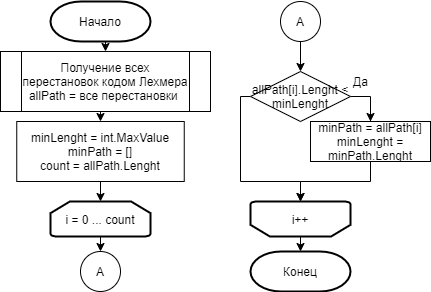
\includegraphics{fullAlgo.png}}
		\caption{Схема алгоритма полного перебора}
		\label{fullAlgo}
	\end{figure}
	\newpage
	\subsection{Схема муравьиного алгоритма}
		На \hyperref[antAlgo]{рисунке  \ref{antAlgo}} изображена схема муравьиного алгоритма.
	\begin{figure}[H]
		\center{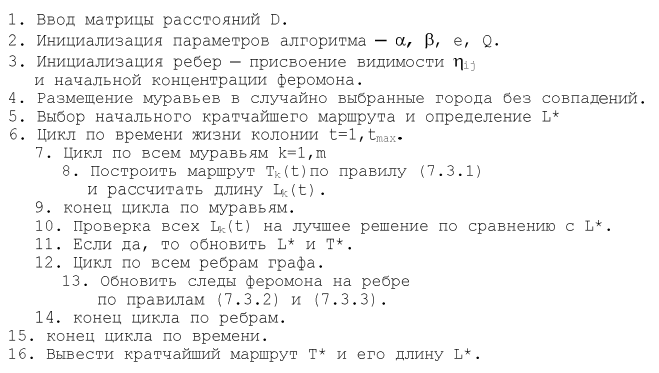
\includegraphics{antAlgo.png}}
		\caption{Схема муравьиного алгоритма}
		\label{antAlgo}
	\end{figure}

	\subsection{Вывод}
	В данном разделе были рассмотрены схемы алгоритмов и обозначены требования к ПО.
	
	\newpage
	\section{Технологическая часть}
	Ниже будут представлены средства реализации и листинги реализованной программы.
	\subsection{Средcтва реализации}
	Выбранный язык программирования - C\#, так как требований по конкретнему языку не выдвигалось и он предоставляет удобные средства распараллеливания.\cite{c-parallel} Среда разработки - Visual Studio.\cite{vs}
\newline
	\indent Технические характеристики машины, на которой проводились тесты:
	\begin{itemize}
	\item Windows 10 x64;
	\item 8 ГБ оперативной памяти;
	\item CPU: AMD FX(tm)-6350 Six-Core Processor 3.90GHz;
	\item 6 логических ядер.
	\end{itemize}	
	\subsection{Реализации алгоритмов}
	Ниже представлены листинги реализаций алгоритмов.
	На листинге \hyperref[fullLst]{\ref{fullLst}} представлен алгоритм полного перебора
	\begin{lstlisting}[label=fullLst, caption=Алгоритм полного перебора]
	static class BruteForce
    {
        public static Path GetMinPath(Graph graph)
        {
            Path shortest = new Path(graph);
            bool isStart = true;
            foreach (Path cur in GetAllRoutes(graph))
            {
                if (isStart)
                {
                    shortest = cur;
                    isStart = false;
                }
                if (shortest.N > cur.N)
                {
                    shortest = cur;
                }
            }
            return shortest;
        }

        private static List<Path> GetAllRoutes(Graph graph)
        {
            int count = graph.count;
            List<Path> routes = new List<Path>();
            List<int> data = new List<int>();
            int[] factorial = new int[count];
            int allSwap = 1;
            for (int i = 0; i < count; i++)
            {
                data.Add(i);
                allSwap *= i + 1;
                factorial[i] = allSwap;
            }

            for (int i = 0; i < allSwap; i++)
            {
                Path curRes = new Path(graph);
                List<int> source = new List<int>(data);
                for (int j = 0; j < count; j++)
                {
                    int p = i / factorial[count - 1 - j] % source.Count;
                    curRes.AddTown(source[p]);
                    source.RemoveAt(p);
                }
                curRes.AddTown(curRes.FirstTown());
                routes.Add(curRes);
            }
            return routes;
        }
	\end{lstlisting}

	\indent На листинге \hyperref[antLst]{\ref{antLst}} представлен муравьиный алгоритм.
	\begin{lstlisting}[label=antLst,caption=Муравьиный алгоритм]
static class AntColonyOptimization
    {
        public static Path GetRoute(Graph graph, int maxTime, double alpha, double beta, double Q, double pho)
        {
            Random r = new Random();

            Path shortest = new Path(graph);
            shortest.distance = int.MaxValue;

            int count = graph.count;
            double[,] pher = InitPheromone(0.1, count);

            for (int time = 0; time < maxTime; time++)
            {
                List<Ant> ants = InitAnts(graph);
                for (int i = 0; i < count - 1; i++)
                {
                    double[,] deltaPher = InitPheromone(0, count);
                    foreach (Ant ant in ants)
                    {
                        int curTown = ant.LastVisited();

                        double sum = 0;
                        for (int town = 0; town < count; town++)
                        {
                            if (!ant.IsVisited(town))
                            {
                                double tau = pher[curTown, town];
                                double eta = 1.0 / graph[curTown, town];
                                sum += Math.Pow(tau, alpha) * Math.Pow(eta, beta);
                            }
                        }

                        double[] probability = new double[count];
                        for (int checkTown = 0; checkTown < count; checkTown++)
                        {
                            double chance = 0;
                            if (!ant.IsVisited(checkTown))
                            {
                                double tau = pher[curTown, checkTown];
                                double eta = 1.0 / graph[curTown, checkTown];
                                chance = Math.Pow(tau, alpha) * Math.Pow(eta, beta) / sum;
                            }
                            probability[checkTown] = chance;
                        }
                        int newTown = GetPosByProb(probability);
                        ant.VisitTown(newTown);
                        deltaPher[curTown, newTown] += Q / ant.GetDistance();
                    }
                    for (int k = 0; k < count; k++)
                    {
                        for (int t = 0; t < count; t++)
                        {
                            pher[k, t] = (1 - pho) * pher[k, t] + deltaPher[k, t];
                            if (pher[k, t] < 0.1)
                            {
                                pher[k, t] = 0.1;
                            }
                        }
                    }
                }
                foreach (Ant ant in ants)
                {
                    ant.VisitTown(ant.Start);

                    if (ant.GetDistance() < shortest.N)
                    {
                        shortest = ant.GetPath();
                    }
                }
            }
            return shortest;
        }
        static int GetPosByProb(double[] probability)
        {
            double[] comulativeProb = new double[probability.Length];
            comulativeProb[0] = probability[0];
            for (int i = 1; i < probability.Length; i++)
            {
                comulativeProb[i] = probability[i] + comulativeProb[i - 1];
            }
            
            Random random = new Random((int)DateTime.UtcNow.Ticks);
            int res = 0;
            double choose = random.NextDouble();
            for (int i = 0; i < comulativeProb.Length; i++)
            {
                if (choose <= comulativeProb[i] && probability[i] != 0)
                {
                    res = i;
                    break;
                }
            }
            return res;

        }

        private static List<Ant> InitAnts(Graph graph)
        {
            List<Ant> ants = new List<Ant>();
            for (int i = 0; i < graph.count; i++)
            {
                ants.Add(new Ant(graph));
                ants[i].VisitTown(i);
            }
            return ants;
        }

        private static double[,] InitPheromone(double num, int size)
        {
            double[,] phen = new double[size, size];
            for (int i = 0; i < size; i++)
            {
                for (int j = 0; j < size; j++)
                {
                    phen[i, j] = num;
                }
            }
            return phen;
        }
    }
	\end{lstlisting}
		
	\subsection{Вывод}
	В данном разделе были описаны программные и аппаратные средства реализации, были представлены листинги реализаций алгоритмов.

	\newpage
	\section{Экспериментальная часть}
	В данной главе будет представлен пример работы программы, результат экспериментов по замеру времени и произведен сравнительный анализ алгоритмов по затрачиваемому времени.
	\subsection{Пример работы программы}
	Пример работы программы представлен на рисунке \hyperref[programmWork]{\ref{programmWork}}
	 	\begin{figure}[h!]
		 	\center{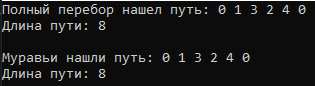
\includegraphics[scale=0.9]{programmWork.png}}
		 	\caption{Пример работы программы}
		 	\label{programmWork}
	 	\end{figure}
	
	\subsection{Сравнительный анализ алгоритмов по времени}
	Были проведены замеры времени работы алгоритмов на количестве вершин от 2 до 10 с шагом 1 и от 10 до 100 с шагом 5. Результаты представлены на рисунке \hyperref[test2]{\ref{test2}}.
	\begin{figure}[h!]
		 	\center{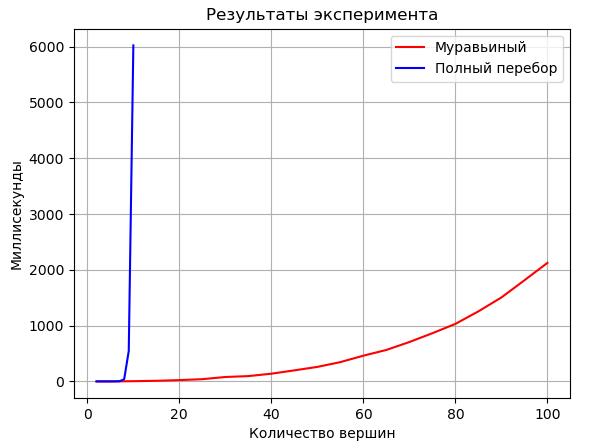
\includegraphics{test2.png}}
		 	\caption{Результаты эксперимента}
		 	\label{test2}
	 	\end{figure}

	\indent Как видно из графиков, муравьиный алгоритм значительно быстрее алгоритма полного перебора. Алгоритм полного перебора уже при 10 вершинах демонстрирует резкий рост времени выполнения, что делает дальнейшее его тестирование слишком затратным по времени. Муравьиный же алгоритм даже при 100 вершинах демонстрирует меньшее время работы, чем алгоритм полного перебора при 10 вершинах.
	
\subsection{Параметризация муравьиного алгоритма}
На рисунках \hyperref[testTOL1]{\ref{testTOL1}}- \hyperref[testTOL30]{\ref{testTOL30}} изображен процент успешного решения задачи в серии из 10 задач в зависимости от варьируемых параметров.

\begin{figure}[H]
		 	\center{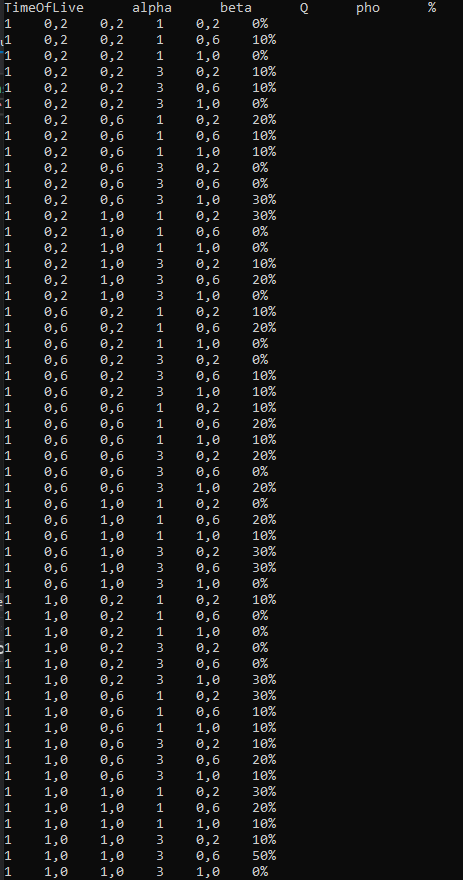
\includegraphics{testTOL1.png}}
		 	\caption{Результаты эксперимента при TimeOfLive = 1}
		 	\label{testTOL1}
	 	\end{figure}
\begin{figure}[H]
		 	\center{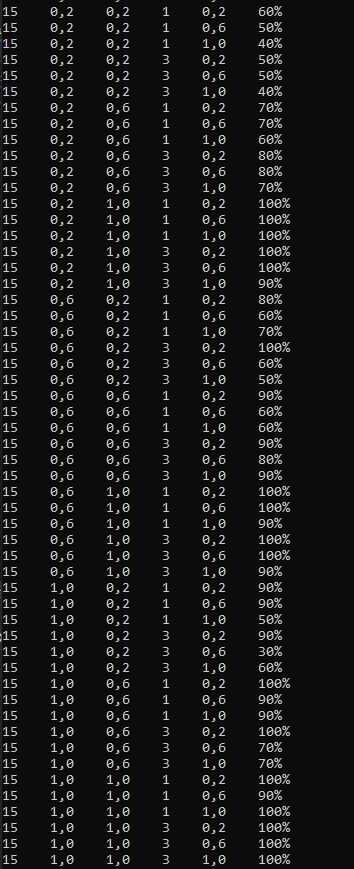
\includegraphics{testTOL15.png}}
		 	\caption{Результаты эксперимента при TimeOfLive = 15}
		 	\label{testTOL15}
	 	\end{figure}
\begin{figure}[H]
		 	\center{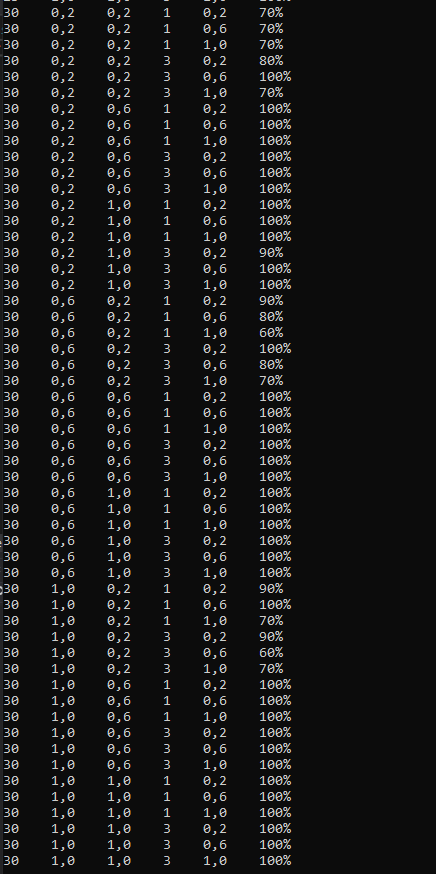
\includegraphics{testTOL30.png}}
		 	\caption{Результаты эксперимента при TimeOfLive = 30}
		 	\label{testTOL30}
	 	\end{figure}

\indent Как видно из результатов, наибольшее влияние на точность алгоритма оказывает TimeOfLive. При равном TimeOfLive, варьирование alpha и beta оказывает второе по величине влияние, phi - третье и Q - четвертое.
	\subsection{Вывод}
	В данной части работы экспериментально было подтверждено значительное превосходство муравьиного алгоритма в скорости работы над алгоритмом полного перебора, была проведена 

	\newpage
	\begin{center}
		\section*{Заключение}
	\end{center}
	\addcontentsline{toc}{section}{Заключение}
	\indent \indent В данной лабораторной работе были разработаны параллельные алгоритмы Винограда. Они были реализованы, а также были проведены эксперименты по замеру времени работы реализованных алгоритмов и проведены сравнения алгоритмов по результатам эксперимента. Цель работы достигнута, все задачи выполнены.
	\newpage
	\addcontentsline{toc}{section}{Список литературы}
	
	\begin{center}
	\begin{thebibliography}{3}
	\bibitem{antAl}
	Муравьиный алгоритм [Электронный ресурс]. Режим доступа: (дата обращения - 01.12.2020) Свободный. URL: http://www.machinelearning.ru/wiki/index.php?title=Муравьиные\_алгоритмы
	\bibitem{c-parallel}
	API.NET. Пространство имен System.Threading [Электронный ресурс]. Режим доступа: (дата обращения - 01.12.2020) Свободный. URL: https://docs.microsoft.com/ru-ru/dotnet/api/system.threading?view=netcore-3.1
	\bibitem{vs}
	Visual Studio [Электронный ресурс]. Режим доступа: (дата обращения - 01.12.2020) Свободный. URL: https://visualstudio.microsoft.com/ru/

	\end{thebibliography}
	\end{center}
\end{document}